% HWI bachelor document template
% author: Prof. Dr.-Ing. Volker Skwarek
% contact: volker.skwarek@haw-hamburg.de
\newcommand{\templateversion}{HWI-Template v5 11.10.2021}
%---------------------------------------

%---------------------------------------
% in order to make this document more readable
% all document setting which better shall NOT
% be changed are moved into the preamble file
%---------------------------------------
% it may happen for compatibility reasons of 
% individually added packagesm that this 
% preamble needs to be changed nevertheless
%---------------------------------------
% but this is, what LaTeX is and it is for...
%---------------------------------------

%---------------------------------------
% variables for document personalisation
%---------------------------------------
\newcommand{\thesistype}{Masterarbeit}
% Bachelorarbeit
% Projektarbeit
% Masterarbeit
% Seminararbeit
% Versuchsbericht
\newcommand{\thesistitle}{Optimization of on-demand line-based bus services}
\newcommand{\student}{Alexander Klaus}
\newcommand{\studentnumber}{7169020}
\newcommand{\firstsupervisor}{Prof. Dr. Knut Haase}
\newcommand{\secondsupervisor}{Prof. Dr. Malte Fliedner}
\newcommand{\thesisdate} {27. August 2025}
%---------------------------------------

\documentclass[
    paper=A4,               % Papierformat
    twoside=false,          % einseitig bedruckt
    fontsize=11pt,          % Schriftgröße
    titlepage=true,         % Titelseite
    listof=totoc,           % Tabellen-/Abb.verzeichnis ins Inhaltsverzeichnis
    bibliography=totoc,     % Literaturverzeichnis ins Inhaltsverzeichnis
    listof=left,            % Tabellen-/Abb.verzeichnis ohne Einzug, hängend
    open=right,             % Kapitel rechts beginnen
    headsepline=true,       % Header mit Linie abtrennen
    footsepline=false,      % Footer nicht mit Linie abtrennen
    captions=tableheading,  % Abstände anpassen, für Captions oberhalb von Tab.
    numbers=noendperiod,    % keine Punkte am Ende von Kapitel-/Anhangnummern
    parskip=half-,          % halber Zeilenabstand zwischen Absätzen
    headings=normal         % Überschriften "normaler" Größe
]{scrbook}

\usepackage{scrhack}    % this package is NOT really required, but it improves the compatibility and the visual appearance of some other packages

%headers right aligned
\usepackage{scrlayer-scrpage}
\automark{chapter}
\clearpairofpagestyles
\setkomafont{pagehead}{\sffamily\small\upshape}
\ohead{\headmark}
\cfoot*{\pagemark}


\usepackage[a4paper]{geometry}
\geometry{
    includehead=true, % wg. fancyhdr-Formatierung zählt Head optisch zum Text
    hmarginratio=1:2, % Rand innen:außen (für Doppelseite ergibt sich: 1:1:1)
    vmarginratio=3:5, % Rand oben:unten (Standard: typearea 1:2, geometry 2:3)
    textwidth=170mm,  % Breite der Textfläche (ohne Randnotizen)
    textheight=230mm, % Höhe der Textfläche (ohne Header)
    headheight=20pt,  % Header größer gegen overfull vboxes (Standard: 12pt)
    footskip=15mm,    % Abstand Baseline des Footer zum Textkörper
    bindingoffset=6mm % Bindekorrektur BCOR
}
\usepackage[utf8]{inputenc} % required for more than the standard english ASCII-7-characters. Or in other words: if you want to type Ä or Ö instead of \"A and \"O, you should keep it
\usepackage[english,ngerman]{babel} % imports hyphenation rules for English and new German spelling rules
\usepackage[T1]{fontenc}	% verbesserte Darstellung von Umlauten
\usepackage{csquotes}   % language dependent quotation marks

\usepackage{xcolor} % required because of HWI specific color settings of the title page
\usepackage{setspace} % also required for the titlepage


\usepackage{graphicx} % required for all kinds of graphics
\usepackage[backend=biber, style=authoryear-icomp, citestyle=authoryear]{biblatex} %set the references and bibliography with the more up-to-date biber than using bibtex
%individual settings in the main document

% set maximum numbering for toc and sections
\setcounter{secnumdepth}{2} % subsection
\setcounter{tocdepth}{2} % subsection
\newcommand{\dottedsection}[1]{#1.}

\raggedbottom % don't stretch incomplete pages to bottom

\usepackage{tabularx} %required for special settings in toc, tof
\usepackage{ifthen} %required for conditional compilation of the latex document specifically for certain types of thesises


% settings for references and bibliography already preloaded in preamble
%here: only individual settings
\ExecuteBibliographyOptions{
    sorting=nyt, %Sortierung Autor, Titel, Jahr
    bibwarn=true, %Probleme mit den Daten, die Backend betreffen anzeigen
    isbn=false, %keine isbn anzeigen
    url=true
}

%-------------------------------------
\addbibresource{your_literature.bib} %Bibliographiedateien laden

%-------------------------------------

%-------------------------------------
% These here are nice additional settings
% which may be changed if required
%-------------------------------------

\usepackage{url}  

%\usepackage{float}
\usepackage{caption}    %captions below figures and tables
    \captionsetup{                  % globale Option für caption und subcaption
      font=normalsize,              % Schrift der Caption (Label+Text)
      format=hang,                  % Formatierung der Caption
      justification=RaggedRight,    % linksbündig bei mehreren caption-Zeilen
      singlelinecheck=true,         % true: einzelne Linie zentriert!
      labelfont=bf,                 % Schrift des Labels
      textfont=rm,                  % Schrift des Textes
      position=bottom               % Normale Caption unter dem Float
    }
\usepackage{subcaption}

\usepackage[colorlinks=true,linkcolor=blue, citecolor=magenta]{hyperref}
\usepackage{booktabs}
\usepackage{acronym} %define acronyms and list them in a glossary
\usepackage{siunitx}[=v2]   % Einheitenmakros, Nummernformatierung
    \sisetup{locale=DE, %Dezimalkomma
    binary-units = true} %Bit als Einheit

\usepackage{blindtext} %can be removed from final document as this is need for the annex in this template document only.
    
    
%-------------------------------------
% The main document starts here
%-------------------------------------
\begin{document}

\frontmatter
%------------------------------------------------------------------------------%
%------------------------------------------------------------------------------%
%--- Titel:    HAW-LaTeX-Vorlage und Hinweise zu studentischen Arbeiten     ---%
%--- Autor:    Rainer Sawatzki <rainer.sawatzki@haw-hamburg.de>             ---%
%---           Hochschule für Angewandte Wissenschaften Hamburg              ---%
%---           Fakultät Life Sciences                                       ---%
%---           Ulmensiet 20, 22033 Hamburg                                  ---%
%--- Vorlage:  Timo Pe <timo.pe@tuhh.de> <mail@timope.com>                  ---%
%------------------------------------------------------------------------------%
%------------------------------------------------------------------------------%

\begin{titlepage}
\definecolor{hwiFarbe}{RGB}{54,170,106}
\sffamily\bfseries % Schriftfamilie
%\onehalfspacing
\doublespacing
	
%------------------------------------------------------------------------------%
%---- Logos und Anschriften ---------------------------------------------------%
%------------------------------------------------------------------------------%

% Der Titel soll, unabhängig der Größe der Logos und Anschriften, immer
% auf gleicher Höhe anfangen. Es wird deshalb eine parbox mit fester Höhe
% als äußeres Konstrukt verwendet.
\begin{minipage}[l][7.5cm][t]{\textwidth}
	\begin{center}
		
\includegraphics[height=3.5cm]{_basic_settings_dont_touch/hwi-logo.jpg} \\	
	\end{center}
\end{minipage}
%------------------------------------------------------------------------------%
%---- Art der Arbeit ----------------------------------------------------------%
%------------------------------------------------------------------------------%

\begin{minipage}[l][5.0cm][t]{\textwidth}
	\begin{center}

		{\Huge
			\textcolor{hwiFarbe}{\thesistype{}} % siehe Beispiele oben
		} \\	[\baselineskip]
	
%------------------------------------------------------------------------------%
%---- Titel -------------------------------------------------------------------%
%------------------------------------------------------------------------------%

		{\Large % Schriftgröße
			\thesistitle			} \\[\baselineskip]
			
%------------------------------------------------------------------------------%
%---- Autor -------------------------------------------------------------------%
%------------------------------------------------------------------------------%
		vorglegt von
		
		{\large % Schriftgröße

			\student \\
			Matrikelnummer \studentnumber
		} \\
	\end{center}
\end{minipage}


%------------------------------------------------------------------------------%
%---- Prüfer, Betreuer, Datum -------------------------------------------------%
%------------------------------------------------------------------------------%

\vfill % dehnbarer vertikaler Abstand, > volle Texthöhe nutzen

\begin{tabular}{@{}ll}
	Bereich: & \\
	1. Gutachter:  & \firstsupervisor \\	
	2. Gutachter:  & \secondsupervisor \\
	vorgelegt am:  & \thesisdate
\end{tabular} \\[-1.0\baselineskip]

\hspace*{.55\linewidth}\begin{minipage}[t][-0.5cm][t]{\textwidth}%
\raggedright
\scriptsize
\singlespacing
\textcolor{gray}{
    \scriptsize
	AM LEHRANGEBOT BETEILIGTE HOCHSCHULEN:\\
	Universität Hamburg\\
	Hochschule für Angewandte Wissenschaften Hamburg\\
	\ifthenelse{\equal{\thesistype}{Bachelorarbeit}}
    {% True case
    }
    {% false case
        Helmut Schmidt Universität - Universität der Bundeswehr Hamburg\\
    }
	%Technische Universität Hamburg-Harburg\\
}
\end{minipage}
\end{titlepage}


\cleardoublepage
\pagestyle{headings}
\tableofcontents
{\let\thefootnote\relax\footnote{\templateversion}}
\listoffigures
\listoftables




\chapter*{Abkürzungsverzeichnis}
\addcontentsline{toc}{chapter}{Abkürzungsverzeichnis}
% Änderungen bezüglich des Plurals sind in der Präambel zu finden
\begin{acronym}

\end{acronym}

\mainmatter
\thispagestyle{plain}
\pagenumbering{arabic}
\chapter{Einleitung}
\section{Einordnung drahtloser Sensornetzwerke}

\ac{DSN}, englisch \ac{WSN} genannt, entstehen durch den Trend des \ac{IoT}, in dem zumindest theoretisch alle Dinge miteinander vernetzt kommunizieren können und somit eine hochdynamisch optimierbare Welt entsteht. Der Ursprung dieser Idee lässt sich bis in die 1990er-Jahre zurück nachvollziehen, in denen Kahn \parencite{Kahn1999} von \emph{smart dust} sprach und somit über einen Begriff das Bild unzähliger kleiner, einfacher, billiger Systemelemente prägte. Diese sollen dann über eine einfache, ursprünglich noch \ac{IP}-basierte Kommunikation miteinander Daten austauschen und eine vernetzte Welt bilden. Das Gegenstück, das die Rechenleistung der vernetzten Welt bereitstellt, bilden dann die Cloud-Systeme mit prinzipiell unbeschränkter Rechenleistung und Kommunikationskapazität.

Gemeinsam bilden diese beiden Systeme das \ac{IoT}, das nach \textcite{InternationalOrganizationforStandardization1997} als 

Internet of Things (IoT):
An infrastructure of interconnected objects, people, systems and information resources together with intelligent services to allow them to process information of the physical and the virtual world and react.

definiert ist. Die \ac{DSN} bilden darin die Anbindung an die reale Welt, liefern als Sensoren Daten oder als aktivieren als Aktoren andere Systeme. Aus dieser Sichtweise werden sie auch als \ac{CPS} bezeichnet und nach Lee \parencite{Lee2008} folgendermaßen definiert

Cyberphysical System (CPS): Cyber-Physical Systems (CPS) are integrations of computation with physical processes. Embedded computers and networks monitor and control the physical processes, usually with feedback loops where physical processes affect computations and vice versa.

Dabei ist zu berücksichtigen, dass das Gebiet der \ac{DSN} \emph{alle} Facetten von Entwurf und Implementierung des Systems abbildet. Ohne Anspruch auf Vollständigkeit der Aufzählung gehören dazu individuelle Aspekte wie Controller, Sensoren, Baugröße und -form aber auch Systemkomponenten wie Übertragungsprotokolle und Kommunikationstopologien oder theoretische Entwurfsparameter, die durch Sicherheits- und Energiebedarfsbetrachtungen geprägt sind. Letztlich nehmen auch Anwendungsaspekte wie ober- oder unterirdischer Einsatzbereich, Ortungsanwendungen oder auch dauerhafter Stand-alone-Betrieb wesentlichen Einfluss auf die Systemauslegung. Damit erfordert der Entwurf drahtloser Sensornetze ein weites Überblickswissen über große Bereiche der Elektrotechnik und der Technischen Informatik sowie über Grundlagen der Physik, der Technischen Mechanik sowie weiterer Ingenieurwissenschaften.  

Im Rahmen dieser Vorlesung wird ein solides Grundwissen in diesen Disziplinen durch eine breite Ingenieurausbildung vorausgesetzt, so dass hier wesentliche Bereiche vertieft werden können. Dabei ist der Begriff \emph{vertieft} auch nur als ein punktuell erweiterter Überblick zu verstehen. 

Die Vorlesungseinheiten beginnen daher mit exemplarischen Anwendungen und leiten daraus spezifische Komponenten und deren besondere Anforderungen an die Funktionsweise ab. Es ergeben sich so spezielle Aspekte zu Kommunikationsverfahren, Netzwerktopologien sowie der Sicherheit. Als besonderer Anwendungsfall werden dann noch die Lokalisierung sowie das Tracking thematisiert, bevor die Vorlesung mit einem Überblick über bestehende Standards auf diesem Gebiet abgeschlossen wird.

Zum Ende der Vorlesung sollten die Studierenden in der Lage sein, 
\begin{itemize}
	\item ein drahtloses Sensornetz anforderungsgerecht auszulegen, 
	\item erforderliche Komponenten und Kommunikationsverfahren zu identifizieren und
	\item sinnvolle Topologien festzulegen,
	\item die den Sicherheitsanforderung und
	\item dem Energiebudget entsprechen.
\end{itemize} 
Als spezieller Anwendungsfall sollen Ortungsverfahren konkret angewendet und umgesetzt werden können.

\section{Grundbegriffe}

Drahtlose Sensornetze bestehen in der Regel nicht aus Einzelkomponenten, sondern bilden ein dem Anwendungsfall entsprechend komplexes Netzwerk. Die einzelnen Endgeräte werden dabei \emph{Knoten} (engl. \emph{\index{nodes}}) genannt und bauen eine drahtlose Verbindung zu einer - wie auch immer gearteten - Infrastruktur auf (s.~Abb.~\ref{fig_wsn_struktur}). 

\begin{figure}[!h]
\centering
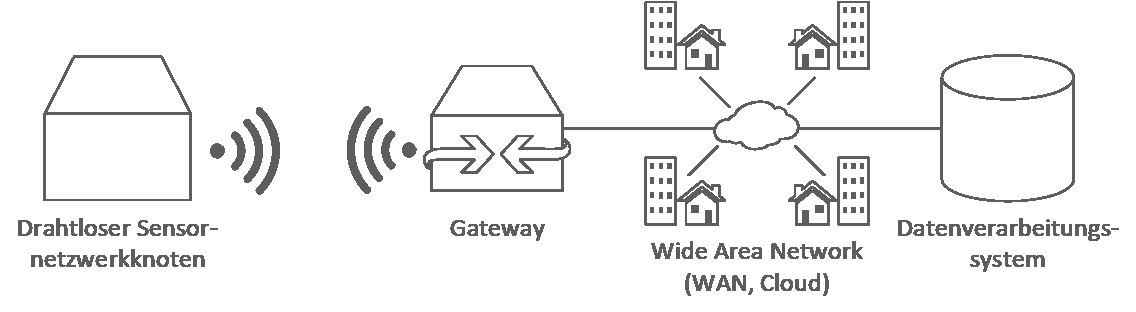
\includegraphics[width=12cm]{your_content_folder/your_figures/fig_intro/WSN_Struktur.png}
\caption{Grundstruktur eines drahtlosen Sensornetzwerkes.}
\label{fig_wsn_struktur}
\end{figure}

Aufgrund der üblicherweise stark eingeschränkten Kommunikationsmöglichkeiten eines solchen \ac{DSN} können diese in der Regel nicht auf ein weitreichendes Übertragungsnetzwerk (\ac{WAN}) mit hohen Bandbreiten zugreifen, sondern benötigen Gateways, die mehrere Netzwerkprotokolle beherrschen und zwischen ihnen übersetzen können. Als Einsatzgebiet wird grob unterschieden zwischen
\begin{description}
	\item [Einzelüberwachung], bei der singuläre Eigenschaften eines Systems wie die Temperatur eines Nahrungsmittels oder die mechanische Spannung einer Brücke aufgenommen wird. Hier liegen eher stationäre Werte vor, die an definierten Stellen entnommen werden und untereinander zu keinen wesentlichen Abweichungen führen. Möglicherweise können mit Hilfe von Modellen sogar eine Plausibilitätsüberprüfung oder eine Redundanzkontrolle vorgenommen werden.
	\item[Bereichsüberwachung], bei der ein unspezifisches Ereignis bzw. ein definiertes Ereignis an einer beliebigen Stelle in einem größeren Bereich aufgenommen werden soll. Hier besteht die Herausforderung darin, die drahtlosen Sensoren so zu verteilen, dass sie in der Lage sind, das Ereignis zu detektieren. Darüber hinaus ist die Anzahl der erforderlichen Sensoren so gering wie möglich zu halten. Trotzdem kann das System zunächst als statisch angesehen werden, und eine Verletzung dieses statischen Zustandes entspräche dann dem zu detektierenden Ereignis.
	\item[Bereichsüberwachung mit Einzeldetektion], bei der beipielsweise ein Bereich auf das Bewegungsverhalten eines Tieres hin überwacht werden soll. Ein solches System stellt die größten Anforderungen an ein Sensornetzwerk, da es hochdynamisch reagieren muss: Sowohl der Bereich, der Detektionspunkt als auch das Objekt sind zunächst unbekannt und müssen aus der Vielzahl der Möglichkeiten erst identifiziert werden, bevor diese dann klassifiziert und analysiert werden können.
\end{description}

Aus diesen generalisierten Einsatzfällen werden unterschiedliche die besonderen Eigenschaften und Anwendungstypen deutlich: Sensornetze sind nicht nur \emph{vernetzte Sensoren} im wörtlichen Sinne, sondern erfüllen ihren Einsatzzweck sogar nur als Netzwerk. Die Sensoren überwachen ihre Umgebung, gleichen gegebenenfalls Informationen mit benachbarten Sensoren ab und bilden redundante Cluster. Zudem werden benachbarte Sensoren auch zur Reichweitenverlängerung der eigenen Kommunikationsdistanz genutzt, indem diese empfangene Nachrichten wiederholen und somit weiterverbreiten. Eine solche Kommunikation wird auch als \emph{Multihopp} bezeichnet (s. Abb. \ref{fig_multihopp}).

\begin{figure}[!ht]
\centering
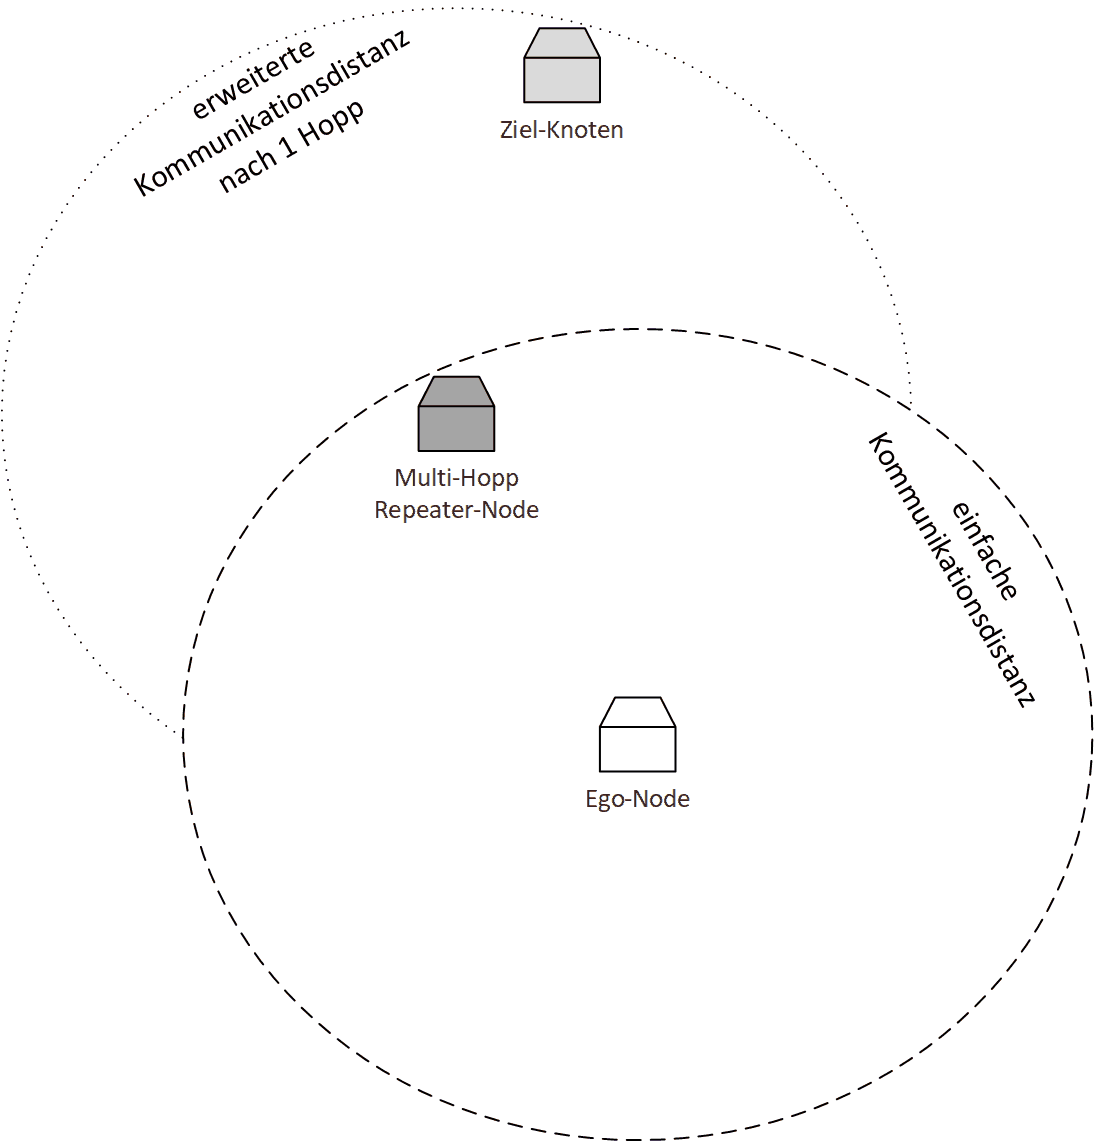
\includegraphics[height=5cm]{your_content_folder/your_figures/fig_intro/Multihopp.png}
\caption{Multihopp-Prinzip der Reichweitenverlängerung.}
\label{fig_multihopp}
\end{figure}

Somit verfügt ein drahtloser Sensorknoten über eine vergleichbar große Aufgabenvielfalt im Vergleich zu den geringen Rechenfähigkeiten und dem stark limitierten Energiebudget.

Entsprechend den Anforderungen des Energiebudgets werden auch spezielle Funkprotokolle zur Kommunikation eingesetzt, die in ihren Eigenschaften den Anwendungsanforderungen angepasst sind: Lange Distanzen werden mit geringer Datenrate beispielsweise über LoRa oder Sigfox überbrückt \parencite{Linklabs2016}, während komfortable, hochratige Verbindungen eher durch Mesh-Netzwerke \parencite{methley_essentials_2009} über sehr kurze Distanzen aufgebaut werden. Industrielle Netzwerke greifen eher auf den IEEE 802.15.4-Standard zurück, während Consumer-Elektronik vorzugsweise Bluetooth verwendet. Wenn wiederum auf den TCP/IP-Protokoll zurückgegriffen werden soll, um eine Internet-Verbindung aufzubauen, kommen in der Regel stationäre Gateways oder Bridges zum Einsatz, die dann über eine umfangreiche Energieversorgung und leistungsfähige Rechner verfügen. Ein Beispiel für ein solches heterogenes Netzwerk ist in Abb. \ref{fig_routed} dargestellt.

\begin{figure}[!ht]
\centering
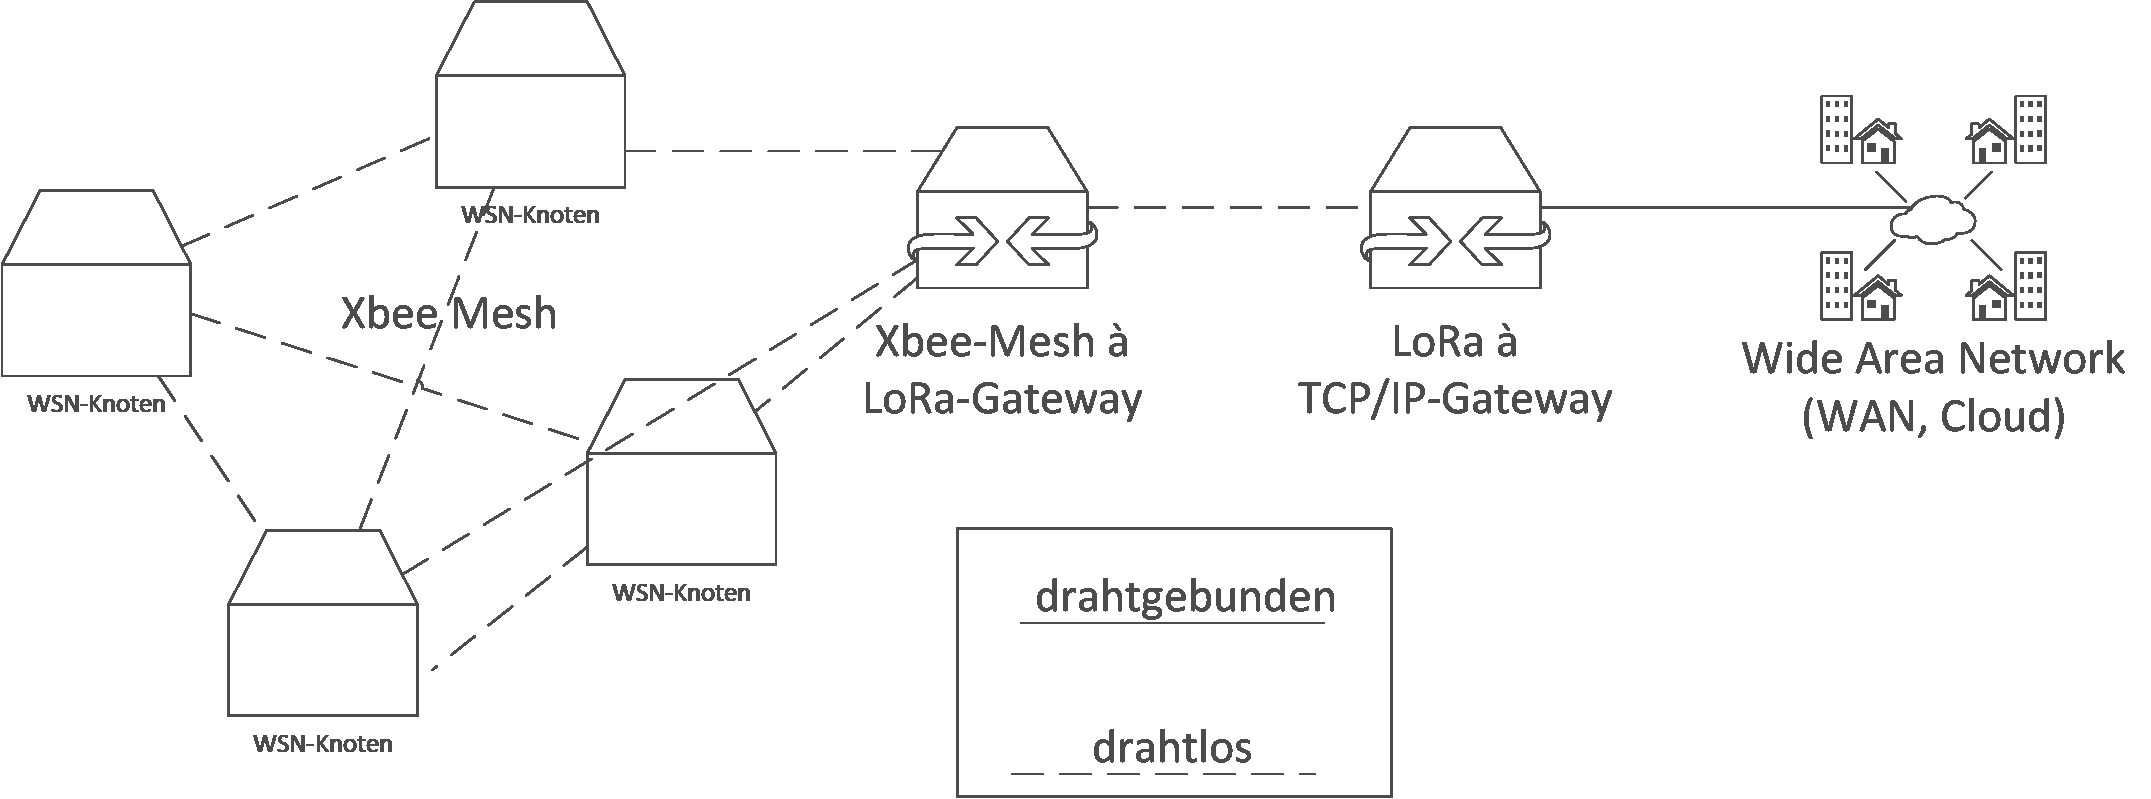
\includegraphics[width=12cm]{your_content_folder/your_figures/fig_intro/Routed_Network.png}
\caption{Beispiel für die Verwendung unterschiedlicher Kommunikationsprotokolle in einem heterogenen Netzwerk mit drahtlosen Sensorknoten.}
\label{fig_routed}
\end{figure}

Als Entwurfsbasis für drahtlose Sensornetzwerke sei also festgehalten, dass diese üblicherweise sehr speziell auf ihre technische Aufgabe ausgelegt werden, um
\begin{itemize}
	\item den Energiebedarf zu minimieren bzw. die Betriebsdauer zu maximieren,
	\item mechanischen Bauraum zu reduzieren,
	\item Stückkosten zu senken.
\end{itemize}
In Abhängigkeit vom Einsatzzweck kann es sogar im Vordergrund stehen, Betriebs- und Ausfallsicherheit durch Redundanz im Netzwerk anstelle einer Überdimensionierung von Einzelkomponenten zu erreichen.

\section{Ursprung von drahtlosen Sensornetzwerken}
Ein Großteil der amerikanischen Literatur \parencite[S.~8]{Dargie2010} oder \parencite[S.~2]{Obaidat2014} benennt militärische Applikationen als Ursprung oder Treiber von drahtlosen Sensornetzwerken. Auch wenn dies möglicherweise einen wahren Kern bilden könnte, so wäre die Sicht zu eingeschränkt, da es sich bei drahtlosen Sensornetzwerken um einen Systemverbund von Komponenten handelt, die evolutionär zu einem Sensornetz zusammengewachsen sind.

Es wäre etwas weit zurückgegriffen, wenn der Ursprung von \ac{DSN} auf die Funkversuche von Nikola Tesla 1893 zurückgeführt würden. Hier wäre fraglich, ob es die Intention von Tesla war, beliebige Knoten oder Systemkomponenten miteinander drahtlos kommunizieren zu lassen. Stattdessen wird in der drahtlosen Kommunikation eher die Entwicklung der internetgebundenen Daten herangezogen. Ursprünglich von der Firma Xerox (1973) mit \SI{2.9}{\mega\bit} entwickelt entstanden dann daraus die Standards IEEE 802.3 für die drahtgebundene und IEEE 802.11 für die drahtlose Internetkommunikation sowie IEEE 802.15.1 für Bluetooth sowie IEEE 802.15.4 für das \ac{WPAN}. Insbesondere das letzte Protokoll ist insbesondere für sehr stabile und energiearme Netze entwickelt worden.

In späteren Kapiteln wird noch intensiver auf die Kommunikation eingegangen. Für das bessere Verständnis ist es aber an dieser Stelle schon sinnvoll kurz das ISO/OSI-7-Schichten Kommunikationsmodell zu erläutern (s.~Abb. \ref{fig_ISO-OSI}):
\begin{figure}[!ht]
\centering
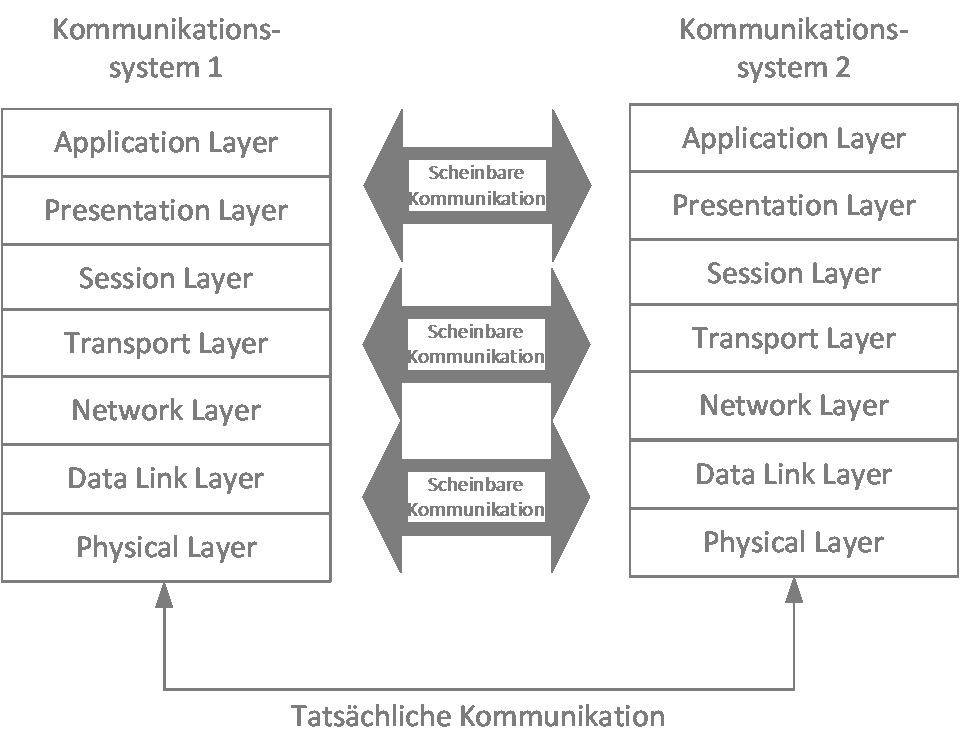
\includegraphics[height=7cm]{your_content_folder/your_figures/fig_intro/ISO_OSI.png}
\caption{ISO-OSI-7-Schichten-Kommunikationsarchitektur.}
\label{fig_ISO-OSI}
\end{figure}
In diesem Modell, das als Referenzmodell für jedes Kommunikationssystem bei ISO oder ITU/T herangezogen wird, sind alle Prozessschritte von der Signalübertragung über ein physikalisches Kommunikationsmedium bis hin zur Datenverwendung in der Nutzeranwendung spezifiziert. Idealweise sollte ein Entwickler beim Senden und Empfangen von Daten nur von einer problemindividuell definierten Schicht in Richtung Applikationsschicht entwickeln müssen. Alle darunterliegenden Schichten sollten idealerweise transparent, also für den Entwickler \emph{unsichtbar} bzw.~nicht von Relevanz sein.

Die oben erwähnten Funkstandards bedienen üblicherweise nur die Schichten 1 bis 2 oder 3, in denen Signale physikalisch generiert, Bits und Bytes zusammengesetzt, ggf. noch ver- oder entschlüsselt oder mit anderen Sicherungsmaßnahmen versehen werden. Hier wird auch von \emph{unteren Protokollschichten} gesprochen.

In den \emph{mittleren Schichten}, also den Schichten 3 bis 5 hingegen werden die Daten zu sinnvollen Worten und Datenpaketen zusammengesetzt, um sie dann anwendungsspezifisch z.~B. als Internetseite oder als Email aufbereiten zu können. 

Die \emph{oberen Schichten} hingegen dienen der anwendungsspezifischen Aufbereitung der Daten.

Ein solches Protokoll in den unteren Schichten für drahtlose Computerkommunikation wurde 1970 von der Universität Hawaii als Aloha-Protokoll veröffentlicht \parencite{Abramson1970, Schwartz2009}. Es handelt sich dabei im Wesentlichen um ein Verfahren zur Kollisionserkennung und Vermeidung bei gleichzeitig sendenden Knoten.

Somit wird die Geburtszeit der drahtlosen Netzwerke auf Anfang der 1970er Jahre datiert. Bevor daraus Sensornetzwerke wurden, waren noch weitere Entwicklungen in der Kommunikationstechnologie sowie in der Größe, der Leistungsfähigkeit und dem Energiebedarf der Controllersysteme erforderlich. Anfang der 2000er-Jahre war eine erste Hype-Phase der Forschung an drahtlosen Sensornetzwerken, in der sich berühmte Forschungsinstitutionen wie die University of California an den Standorten Berkeley und Los Angeles oder das MIT, die sich mit der Entwicklung von der Hardware drahtloser Sensornetze beschäftigt haben. Stichworte über Forschungsergebnisse sind hier \emph{Wireless Integrated Network Sensors (WINS)}, einem ersten sogenannten \ac{CPS}, also einer Einheit, die Daten aufnehmen, verarbeiten und weitergeben kann. Alle diese Einheiten wurden in dem WINS-Projekt auf einem einzigen Chip zusammengefasst.

In Berkeley hingegen wurde das Konzept der Hochintegration auf Komponentenbasis verfolgt. Hier wurde beispielsweise der Begriff \emph{smart dust} \parencite{Kahn1999} als Vorläufer des Internet-of-Things geprägt. Die sehr kleinen Sensoren wurden auch \emph{motes}\footnote{\url{https://computer.howstuffworks.com/mote4.htm}} genannt.

Moderne Knoten drahtloser Sensornetzwerke sind hochintegrierte Rechen- und Kommunikationssysteme auf einem einzelnen Chip. Bei einem Spannungspegel herunter von bis zu $\SI{1.8}{\volt}$ einen Energiebedarf von $\SI{50}{\micro\watt\per\mega\hertz}$ aufweisen bzw.~mit $\SI{1}{\milli\watt}$ kommunizieren.

Das Industriekonsortium EEMBC führt unterschiedlichste Benchmarks durch. Einer dieser Benchmarks ist ein Ultra-Low-Power-Benchmark\footnote{\url{http://www.eembc.org/ulpbench/index.php}}, siehe Abbildung \ref{fig_ulp_bench}. Der pp-Benhmark stellt dabei ein Maß für den Kehrwert die Durchschnittsleistung dar.

Genauer: $\frac{1000}{\text{Median der mittleren Sekundenleistung über 10 Benchmarkzyklen}}$. In dem abgebildeten Benchmark führen die energieeffizientesten Controller die Benchmarkaufgaben folglich bei ca.~$10\ldots \SI{20}{\micro\watt}$ durch.

Hier ist anzumerken, dass dieser Benchmark nicht unumstritten ist, da alle Hersteller gemeinschaftlich festlegen, welche Rechenaufgaben zur Ermittlung des Benchmarkwertes durchgeführt werden. Folglich ist es fraglich, ob dieser Benchmark sehr repräsentativ für einen echten Betrieb ist.

\begin{figure}[!ht]
\centering
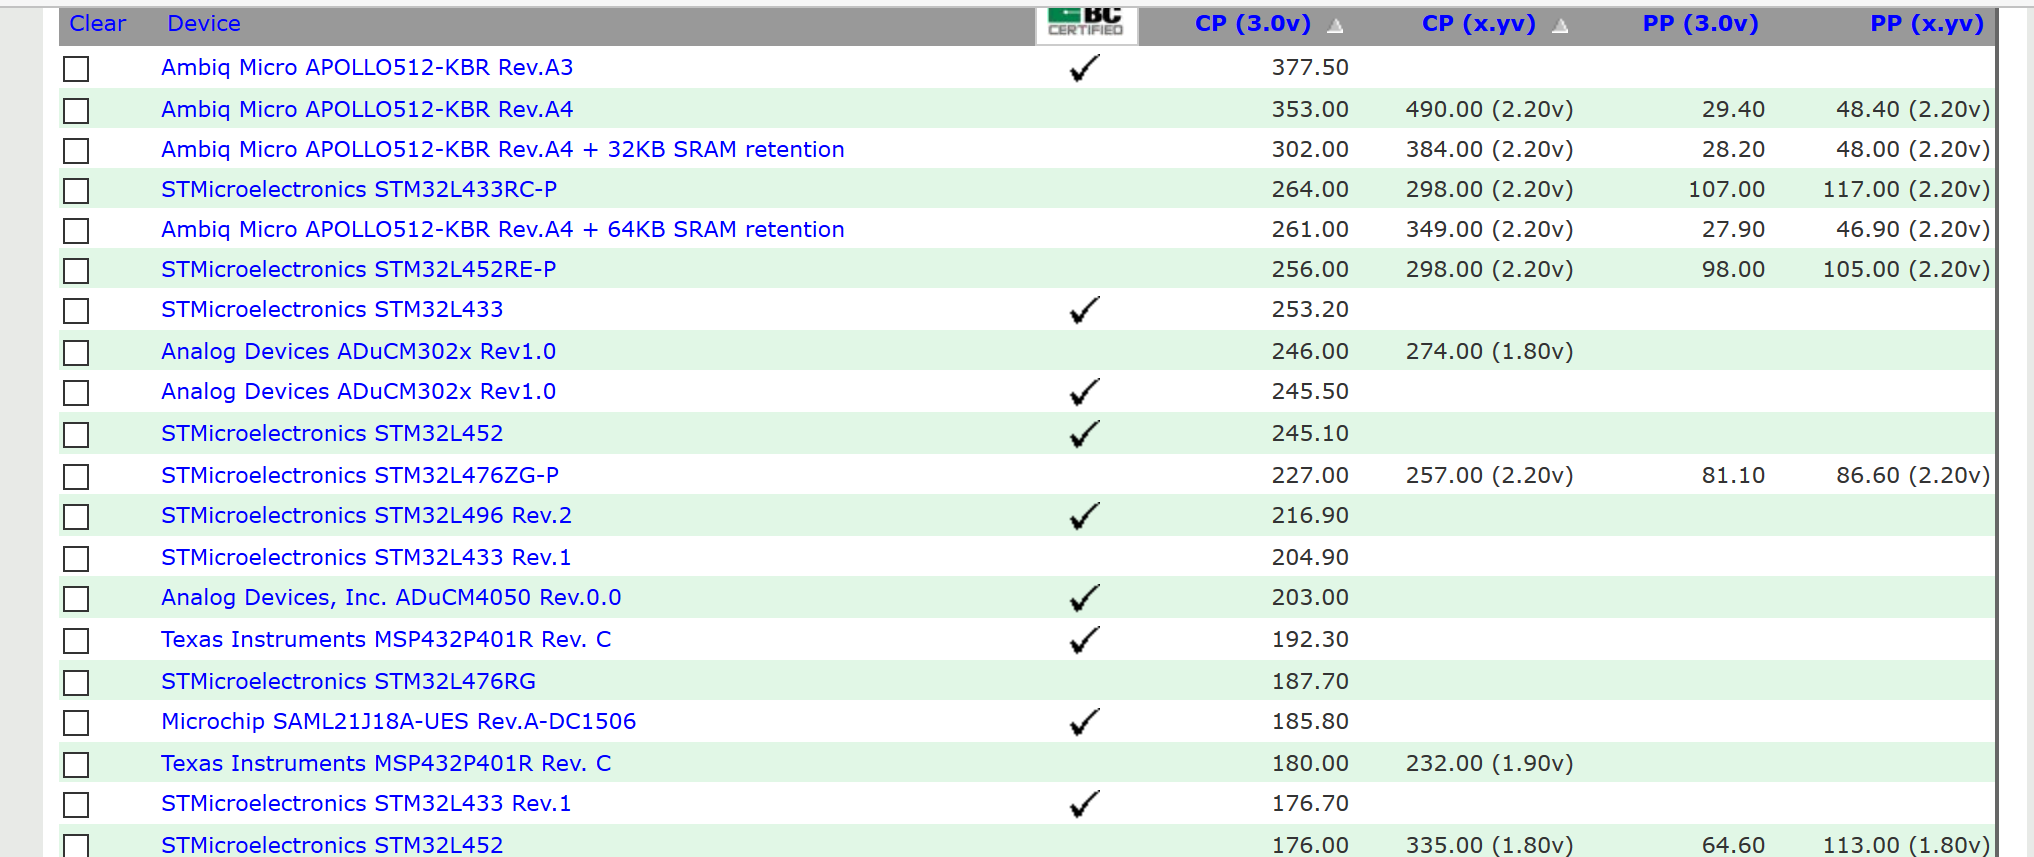
\includegraphics[width=12cm]{your_content_folder/your_figures/fig_intro/ulp_bench.png}
\caption{Ergebnisse des Ultra-Low-Power-Benchmarks von EEBMC, Quelle: \url{http://www.eembc.org/ulpbench/index.php} vom 16.10.2017}
\label{fig_ulp_bench}
\end{figure}

\section{Anwendungsfälle und abgeleitete Eigenschaften}
\subsection{Beispielanwendungen}
Die Anwendungsfälle von drahtlosen Sensornetzwerken sind zahllos und lassen sich kaum klassifizieren. Daher werden im folgenden eher große Anwendungsbereiche mit spezifischen Besonderheiten exemplarisch genannt, um daran später Anforderungsbereiche für Sensornetze festzumachen.



\subsection{Entwurfseigenschaften}

Aus den Anwendungsfällen oben wird ersichtlich, dass ein Sensorknoten üblicherweise lassen sich folgende Entwurfseigenschaften ableiten:

\begin{description}
	\item [Aufgabenbezogenheit] Ein Sensornetz üblicherweise minimalistisch ausgelegt, orientiert sich daher hinsichtlich Prozessorleistung, Speicherkapazität, Batteriekapazität, Nachladeverfahren (= energy harvesting) eng an den Anforderungen. Beispielsweise benötigt ein FRAM zur dauerhaften Speicherung von Daten mehr Energie als ein konventioneller RAM-Baustein. Dies kann allerdings ein lohnenswerter Energieeinsatz sein, wenn der Sensorknoten über lange Pausenzeiten verfügt oder die Versorgungsenergie spontan ausfallen könnte. Der Energiebedarf kann unter anderem durch folgende Maßnahmen gesenkt werden:
	\begin{itemize}
		\item intelligenter Wechsel aus Schlaf- und Arbeitsphasen der einzelnen Netzwerkknoten (engl. duty cycle),
		\item kurze Übertragungszeiten und -strecken. Während die Übertragungszeit nur linear in den Energiebedarf eingeht, muss die Übertragungsdistanz quadratisch berücksichtigt werden. Dies ist darin begründet, dass sich die Funkwelle bei einem ungerichteten Strahler in rotatorischer Form ausbreitet - z.~B.~ einer Kugel -, deren Oberfläche quadratisch mit dem Radius zunimmt.
		\item effiziente, optimierte Netzwerkprokolle mit geringem Datenoverhead, Vermeidung von Kommunikationskollisionen und optimalen Übertragungswegen und
		\item effiziente Programmierverfahren, kleine Betriebssysteme, geringe Prozessorgeschwindigkeit.
	\end{itemize}
	
	\item [Netzwerkorientierung] Das Sensornetz erfüllt seine Aufgabe im Netzwerk und nutzt daher aktiv die Netzwerkeigenschaften. Hierzu gehören neben der Möglichkeit einer vermaschten Kommunikation (mesh-network) auch Ortung und Tracking durch Netzwerkeigenschaften, spezialisierte Aufgaben einzelner Netzwerkknoten, extensive Schlafintervalle einzelner Teilnehmer bei voller Funktion des gesamten Netzwerkes durch Redundanz. Daher ist die Netzwerktopologie ein Kernentwurfskriterium.
	\item [konstruktive Anforderungen der Einsatzumgebung] Sensornetze erfordern aufgrund ihrer Entwurfsminimalität ein Zusammenspiel aller Komponenten aus Software, Hardware und Konstruktion (engl.: \emph{mechanical design}). So könnte beispielsweise ein Sensor zur Messung eines Flüssigkeitsfüllstandes davon technisch profitieren, dass die Flüssigkeit erst durch einen Trichter in einen kleinen Vorratsbehälter läuft und somit Schwingungen und Vibrationen kompensiert werden. Dies erspart dann Soft- und Hardwareverfahren zur Filterung der Messwerte.
	\item [(Vor-)Verarbeitungsanforderungen] Jegliche Verarbeitungsverfahren der Daten sollten sich auf ein Minimum reduzieren, da jeder Rechenvorgang Energie benötigt. Zudem ist auch zu bedenken, dass Niedrigenergiecontroller nur über minimale Prozessorhardware beispielsweise sogar ohne Fließkommaeinheit verfügt.
	\item [operative Autarkie] Sensoren in einem drahtlosen Sensornetz müssen nicht nur energetisch, sondern auch operativ autark agieren. Dies bedeutet, dass wesentliche Systemfunktionen unabhängig von der exakten räumlichen Anordnung zueinander bzw\. unabhängig von einer möglichen Mobilität der Sensoren eingerichtet und ausgeführt werden können müssen. Hierzu zählen beispielsweise der Aufbau und der Betrieb des Netzwerkes selbst, (Netzwerk-) Routingverfahren unter Einbeziehung der Sensornachbarschaft, Anpassung der Betriebsparameter an die Umgebung ohne manuelle Interaktion.
	\item[Zugriffs- und Betriebssicherheit] Die Begriffe werden im Englischen besser durch \emph{security} als Zugriffssicherheit und \emph{safety} als Betriebssicherheit unterschieden. Beide Eigenschaften sind wichtig, um eine zuverlässige Datenübertragung sicherzustellen. Allerdings bedürfen sie ob algorithmischer, verschlüsselnder oder kryptographischer Verfahren, die die Rechenbelastung und somit den Energiebedarf des Sensorknotens stark erhöhen. Daher sind die drahtlosene Sensorknoten oft deutlich weniger leistungsfähig und weitaus anfälliger gegenüber Sicherheitsangriffen.
\end{description}

Über die übliche Grobklassifikation von Sensornetzwerken in der Literatur nach Netzwerkorganisation und Knotenstruktur hinaus lassen sich zahlreiche detailliertere Parameter zur Unterscheidung und Bewertung von Sensornetzen definieren:
\begin{itemize}
\item räumliche Auflösung (spatial resolution),
\item Übertragungsverzögerung von Nachrichten, auch \emph{Latenzzeit} genannt,
\item räumliche Abdeckung (coverage) $C$ als Verhältnis der Gesamtüberwachungsfläche $A_{ges}$ und der durch Sensoren sensierten Fläche $A_{sens}$ mit 
\begin{equation}
	C = \frac{A_{sens}}{A_{ges}},
\end{equation}
\item Art der Systemsteuerung (control) wie zentral, verteilt oder chaotisch,
\item zeitliche Auflösung,
\item Betriebsdauern - im englischen besser differenziert als \emph{lifetime}, also die absolute gesamte Lebensdauer, und \emph{operating time}, also die Betriebsdauer,
\item erforderliche Bandbreite zur Datenübertragung beispielsweise in $\SI{}{\bit\per\second}$ oder $\SI{}{\mega\bit\per\second}$.
\end{itemize}

\section{Aufgaben}
\begin{enumerate}
\item Informieren Sie sich über das Aloha-Protokoll und studieren Sie Varianten davon, z.~B. \emph{unsynchronisiertes (=\,pure) Aloha} und \emph{synchronisiertes (=\,slotted) Aloha}. 
\parencite{Roberts1975}
\item Charakterisieren Sie für drahtlose Sensorknoten die technischen Entwurfsmerkmale Skalierbarkeit, Energiebedarf, Verteilung/Topologie/Abdeckung, Kommunikation und Sicherheit kurz jeweils in ein bis zwei Sätzen.
\item Überlegen Sie sich eine Messaufgabe, bei der Sie drahtlose Sensornetzwerke einsetzen würden. Versuchen Sie insbesondere, eine Anwendung zu finden, bei der gerade der Charakter des "verteilten Netzwerkes", also der kleinteiligen, redundanten Messung genutzt wird.
\item Wie unterscheiden sich Xbee, Zigbee und das IEEE 802.15.4-Protokoll?
\item Wofür wird der IEEE 1451-Standard eingesetzt?
\item Stellen Sie von den Firmen Texas Instruments und ST Microeletronics die Prozessoren der Serien MSP 432 (TI) und STM32 L und F gegenüber tabellarisch hinsichtlich ihrer On-Chip-Hardware und ihrer Energiebedarfe gegenüber.
\item Welche Methoden kennen Sie, um den Energiebedarf von drahtlosen Sensorknoten zu reduzieren?
\item Beschreiben Sie Unterschiede in Single-Hopp- und Multi-Hopp-Kommunikationsverfahren hinsichtlich Energiebedarf, Datendurchsatz, Zuverlässigkeit, Sicherheit und Kommunikationsverzögerungen.
\end{enumerate}

 

\printbibliography 
% do not change: sets specific page numbering for annex
\pretocmd{\chapter}{
    \clearpage
    \setcounter{page}{1}
}{}{}
\let\oldpagestyle=\thepage
\renewcommand*{\thepage}{\thechapter-\arabic{page}}
%----------------------------------------------------

% add annexures here
\appendix
\chapter{Beispielanhang}

\blindmathpaper

\chapter{Zweiter Beispielanhang}


\Blindtext[3]


%--------------------------------------
% you shouldn't make any changes from here
%--------------------------------------

\clearpage
\renewcommand*{\thepage}{\oldpagestyle}
%------------------------------------------------------------------------------%
%------------------------------------------------------------------------------%
%--- Titel:    HWI-LaTeX-Vorlage und Hinweise zu studentischen Arbeiten     ---%
%--- Autor:    Rainer Sawatzki <rainer.sawatzki@haw-hamburg.de>             ---%
%---           Hochschule für Angewandte Wissenschaften Hamurg              ---%
%---           Fakultät Life Sciences                                       ---%
%---           Ulmenliet 20, 22033 Hamburg                                  ---%
%--- Vorlage:  Timo Pe <timo.pe@tuhh.de> <mail@timope.com>                  ---%
%------------------------------------------------------------------------------%
%------------------------------------------------------------------------------%

%\chapter*{Eidesstattliche Erklärung}
\chapter*{Versicherung über die Selbstständigkeit}
 
\thispagestyle{empty}
% Achtung: Für Seminararbeiten ist keine eidesstattliche Erklärung notwendig. In der HWI-template.tex die Datei auskommentieren!

Hiermit erkläre ich an Eides statt, dass ich die vorliegende \thesistype{} ohne fremde Hilfe selbstständig verfasst habe. Ich habe keine anderen als die angegebenen Hilfsmittel -- insbesondere keine im Quellverzeichnis nicht benannten Internet-Quellen -- benutzt. Ich habe die Arbeit vorher nicht in einem anderen Prüfungsverfahren eingereicht. Die schriftliche Fassung entspricht der auf dem elektronischen Speichermedium. \\[2cm]

\begin{tabularx}{\linewidth}{X l X}
	Hamburg, den \today & \hspace*{2cm} & \\
      \cline{1-1}
      \cline{3-3}
      Ort, Datum   &  & Unterschrift \\  % Hier Datum des Druckes bzw. der Abgabe eintragen
\end{tabularx}


\end{document}
